\documentclass[tikz,convert={outfile=\jobname.svg}]{standalone}
\usepackage{tikz}
\usepackage{pagecolor}
\pgfdeclarelayer{background}
\pgfdeclarelayer{foreground}
\usetikzlibrary{shapes.geometric}
\pgfsetlayers{background,main,foreground}
\pagecolor{white}

\tikzset{ 
   line/.style ={
      -, line width=0.5mm, bend angle=90, color=black,
   },
   arrow/.style ={
      ->, line width=0.5mm, bend angle=90, color=black,
   },  
}

\begin{document}
   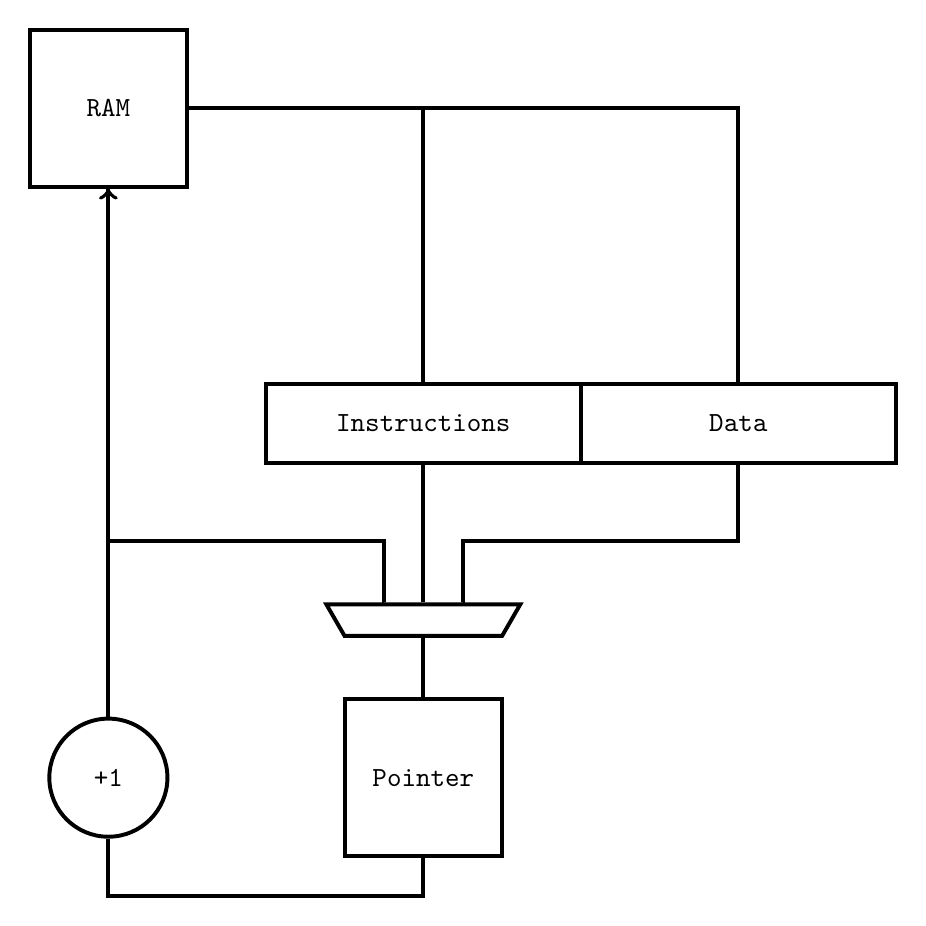
\begin{tikzpicture} 
     
      \node[
         rectangle,
         draw,
         font=\ttfamily,
         line width = 0.5mm,
         minimum height=20mm,
         minimum width=20mm,
      ] (ram) at (-70mm,50mm){RAM};

     \node[
         rectangle,
         draw,
         font=\ttfamily,
         line width = 0.5mm,
         minimum height=10mm,
         minimum width=40mm,
      ] (inst) at (-30mm,10mm){Instructions};

      \node[
         rectangle,
         draw,
         font=\ttfamily,
         line width = 0.5mm,
         minimum height=10mm,
         minimum width=40mm,
      ] (data) at (10mm,10mm){Data};
 
      \node [
         trapezium,   
         draw,   
         shape border rotate = 180,  
         line width = 0.5mm,
         inner xsep=10mm,
         inner ysep=2mm,
      ] (mux) at (-30mm,-15mm) {};
        
      \node[
         rectangle,
         draw,
         font=\ttfamily,
         line width = 0.5mm,
         minimum height=20mm,
         minimum width=20mm,
      ] (ptr) at (-30mm,-35mm){Pointer};

      \node[
         circle,
         draw,
         font=\ttfamily,
         line width = 0.5mm,
         minimum height=15mm,
         minimum width=15mm,
      ] (adder) at (-70mm,-35mm){+1};



      \draw[line] (adder.north) |- (-35mm,-5mm)  |- ([yshift=0mm,xshift=-5mm]mux.north);
      \draw[line] (inst.south)  |- (mux.north);
      \draw[line] (ptr.south)   |- (-70mm,-50mm) |-(adder.south);
      \draw[line] (data.south)  |- (-25mm,-5mm) |-([yshift=0mm,xshift=5mm]mux.north);
      \draw[line] (mux.south)   |- (ptr.north);  
      \draw[arrow] (adder.north) |- (ram.south);
      \draw[line] (ram.east)    |- (-30mm,50mm) |- (inst.north);
      \draw[line] (ram.east)    |- (10mm,50mm) |- (data.north);

   \end{tikzpicture}
\end{document}
